\section{Operaciones Básicas}
\label{sec:basic-operations}

\begin{frame}[fragile]{Repaso de Álgebra Lineal}
  \begin{columns}[t]
    \column{0.2\textwidth}
    \begin{itemize} \justifying \parskip3mm
  \item<only@1-3> Escalar
  \item<only@1-3> Vector
  \item<only@1-4> Matriz
  \item<only@1-4> Tensor
  \end{itemize}

  \column{0.8\textwidth}
  {\centering
    \includegraphics<1>[scale=0.4]{scalar-vector-matrix}
    \includegraphics<1>[scale=0.5]{tensor_shape}
    
    \includegraphics<1>[scale=0.5]{tensor}
    \par}

  \begin{onlyenv}<2>
    \begin{ipythonnb}[1]
import numpy as np
    \end{ipythonnb}
    
    \begin{ipythonnb}
x = np.array(12)
x.ndim
    \end{ipythonnb}
    \begin{ipythonnb2}
0
    \end{ipythonnb2}
\end{onlyenv}

  \begin{onlyenv}<3>
      \begin{ipythonnb}
x = np.array([12, 3, 6, 14, 7])
x
\end{ipythonnb}

\begin{ipythonnb2}
array([12,3,6,14,7])
\end{ipythonnb2}

\begin{ipythonnb}
x.ndim
\end{ipythonnb}

\begin{ipythonnb2}
  1
\end{ipythonnb2}

\end{onlyenv}

  \begin{onlyenv}<4>
    \begin{ipythonnb}
x = np.array([[5, 78, 2, 34, 0],
              [6, 79, 3, 35, 1],
              [7, 80, 4, 36, 2]])

x.ndim
\end{ipythonnb}

      \begin{ipythonnb}
        tensor = np.array([
        [[5, 78, 2, 34, 0],
         [6, 79, 3, 35, 1],
         [7, 80, 4, 36, 2]],
        [[5, 78, 2, 34, 0],
         [6, 79, 3, 35, 1],
         [7, 80, 4, 36, 2]],
        [[5, 78, 2, 34, 0],
         [6, 79, 3, 35, 1],
         [7, 80, 4, 36, 2]]
        ])
\end{ipythonnb}
\end{onlyenv}

  \end{columns}
\end{frame}

\begin{frame}{Vector y Escalar}
  \begin{block}{Vector} \justifying
    Es una magnitud cuya determinación exige el conocimiento de un módulo, una dirección y un sentido. Ejemplos de magnitudes vectoriales son el desplazamiento, la aceleración, la fuerza, etc.
  \end{block}
  \begin{block}{Escalar} \justifying
    Es una magnitud cuya determinación solo requiere el conocimiento de un número, su cantidad respecto de cierta unidad de medida de su misma especie. Ejemplos típicos de escalares son la longitud, la masa, el tiempo, la temperatura, el trabajo, la energía, etc., y cualquier número real.
  \end{block}

  {\centering
    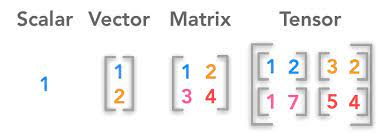
\includegraphics[scale=0.4]{vector}
  \par}
\end{frame}

\begin{frame}[fragile]{Álgebra Lineal Con Python}
  \begin{onlyenv}<1>
      \begin{lstlisting}
    % matplotlib inline
    import matplotlib.pyplot as plt
    plt.imshow(tensor, interpolation='nearest')
    plt.show()
  \end{lstlisting}
\end{onlyenv}

\begin{onlyenv}<2>
  \begin{lstlisting}
tensor = np.array([
		   [[0,0,0,0],  [0,0,0,0], [0,0,0,0]],
		   [[128,128,128], [128,128,128],[128,128,128]],
		   [[255,255,255], [255,255,255], [255,255,255]]
		   ])              

plt.imshow(tensor, interpolation='nearest')
plt.show()
  \end{lstlisting}
               \end{onlyenv}

\end{frame}


\begin{frame}{Repaso de Álgebra Lineal}
  Una embotelladora de refrescos desea cotizar la publicidad de sus productos en televisión,
radio y revista, se tienen tres propuestas del plan de medios de acuerdo con el presupuesto
asignado acerca de la cantidad de anuncios por medio en el transcurso de un mes. En el
primer presupuesto cada anuncio en televisión tiene un coste de \$250 000, en radio \$5 000
y en revista \$30 000. En el segundo presupuesto \$310 000, \$4 000 y \$15 000 y en el último
presupuesto \$560 000, \$10 000 y \$35 000. Los totales por presupuesto son los siguientes:
\$21 795 000, \$31 767 000 y \$61 225 000.
\end{frame}

\begin{frame}{Dimensión de un vector}
  
  \lstinputlisting{scriptsLinAlg/01_dimension_vectors.py}
\end{frame}



\begin{frame}[t]{Transponer, suma de matrices y escalares}
  \begin{onlyenv}<1>
      \lstinputlisting{scriptsLinAlg/02_transpose_sum.py}
    \end{onlyenv}

    \begin{onlyenv}<2>
            \lstinputlisting{scriptsLinAlg/02_sum.py}
    \end{onlyenv}
  \end{frame}

  
%%% Local Variables:
%%% mode: latex
%%% TeX-master: "../slides"
%%% End:
